%===============================================================================
\begin{frame}[t]
\frametitle{Описание эксперимента}
\begin{itemize}
    \item Набор данных MNSIT (10 тыс. изображений рукописных цифр $28 \times 28$)
    \item Данные подаются последовательно из процессорной системы
    \item Результаты группируются в виде матриц спутывания
    \item Проведено 15 тестов с различными разрядностями весовых коэффициентов (от 2 до 16)
    \item Составлен график зависимости точности от разрядности
    \item Разложены классы весовых коэффициентов на битовые плоскости
    \item Проанализированы аппаратные затраты
\end{itemize}

\end{frame}

%===============================================================================
\begin{frame}[t]
\frametitle{Результаты}
\begin{columns}
% \hspace{5mm}
\column[t]{0.45\textwidth}
% \begin{center}
\begin{block}{ \centering Матрица спутывания}
    \vspace{3mm}
    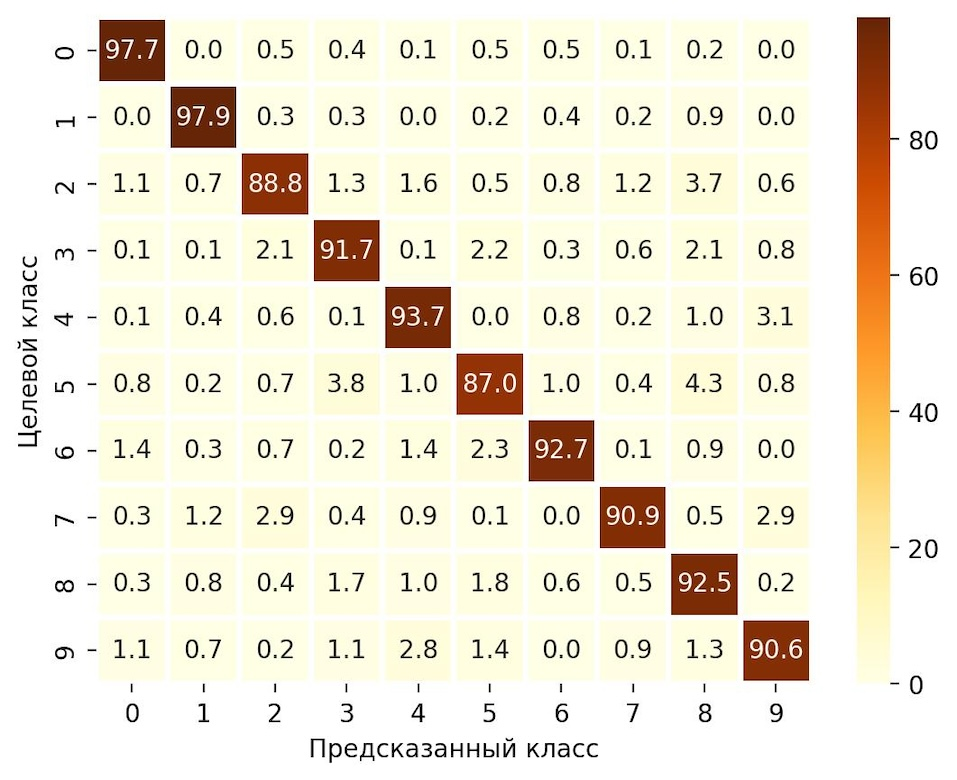
\includegraphics[width = 0.815\textwidth]{pics/cm_6q5.jpg} 
\end{block}
% \end{center}
 
\column[t]{0.45\textwidth}
\begin{block}{\centering Точность и затраты блоков LUT/FF}
    \vspace{3mm}
    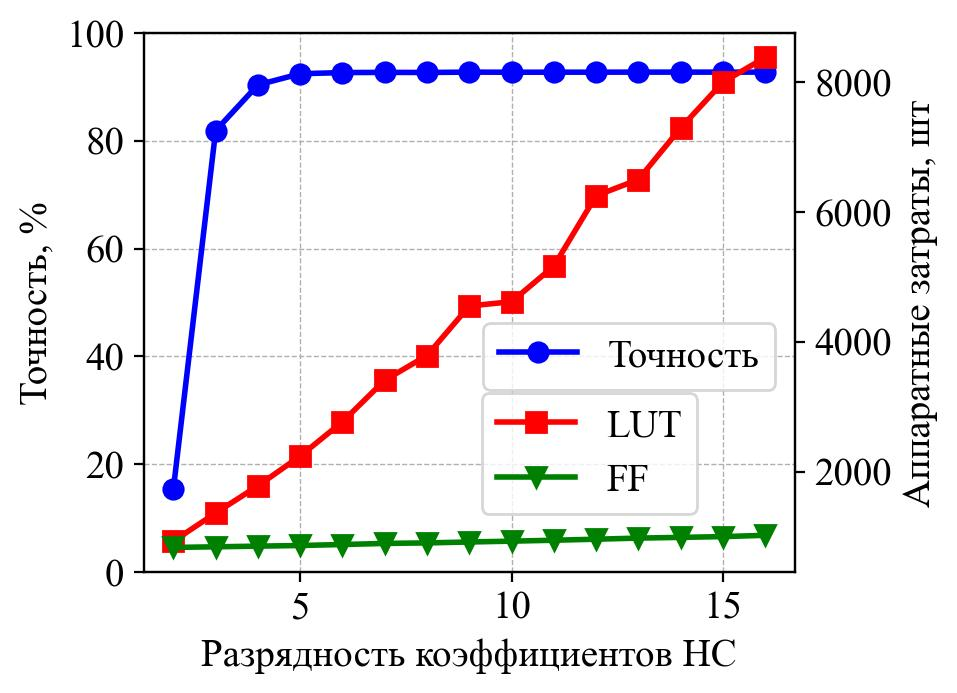
\includegraphics[width = 0.9\textwidth]{pics/Acc_LUTs_FFs.jpg} 
\end{block}

\end{columns}
\end{frame}

%===============================================================================
\begin{frame}[t]
\frametitle{Разложение на битовые плоскости}
\begin{columns}
    \hspace{5mm}
    \column[t]{0.3\textwidth}
    \centering 
    \begin{block}{\centering{Весовой класс 3}}
        \vspace{3mm}
        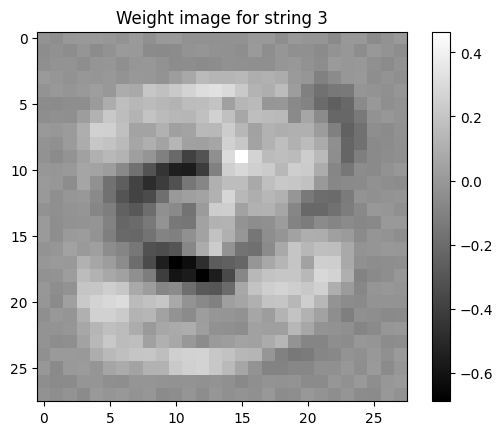
\includegraphics[width = 0.85\textwidth]{pics/output1.png} 
    \end{block}
     
    \column[t]{0.7\textwidth}
    \centering 
    \begin{block}{\centering{Битовые плоскости}}
        \vspace{3mm}
        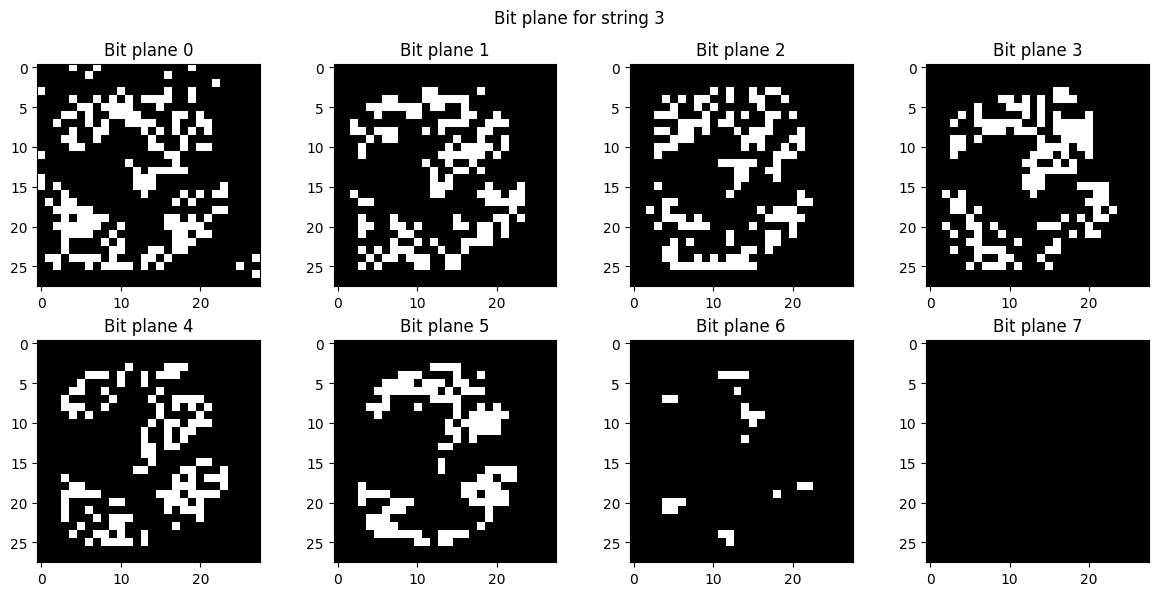
\includegraphics[width = 0.85\textwidth]{pics/output.png} 
    \end{block}
\end{columns}
\end{frame}

%===============================================================================
\begin{frame}[t]
    \frametitle{Аппаратные затраты}
    \centering
    \begin{table}[h]
        \centering
        \caption{Аппаратные затраты для 5 битного представления коэффициентов}
        \begin{tabular}{|>{\raggedright\arraybackslash}p{4cm}|>{\centering\arraybackslash}p{2.5cm}|>{\centering\arraybackslash}p{2.5cm}|>{\centering\arraybackslash}p{2.5cm}|}
            \hline
            Тип блока & Использовано & Доступно & Соотношение, \% \\
            \hline
            LUT as logic & 2180 & 17600 & 12.39 \\
            \hline
            LUT as memory & 60 & 6000 & 1 \\
            \hline
            Flip Flop & 862 & 35200 & 2.45 \\
            \hline
            RAMB18  & 10 & 120 & 8.33 \\
            \hline
            DSP & 0 & 80 & 0 \\
            \hline
            BUFG & 1 & 32 & 3.13 \\
            \hline
        \end{tabular}
    \end{table}
\end{frame}

%===============================================================================
\begin{frame}[t]
\frametitle{Выводы}
\begin{itemize}
    \item Рассмотренный эксперимент на основе НС прямого распространения с
    полносвязным слоем показывает, что формат представление 
    весовых данных существенно влияет на точность определения 
    до 5 битной разрядности. Дальнейшее увеличение разрядности 
    не несет значительных изменений в точности.
    \item Предложенная структура НС показывает, что при увеличении
    разрядности наблюдается линейный рост в потреблении LUT и FF блоков FPGA.
\end{itemize}
\end{frame}

%===============================================================================
% \begin{frame}
%     % \printbibliography
% \end{frame}
